% ch-a4-10.tex —— 第 4 篇（Emerton–Gee–Hellmann）续片，底本 PDF 288–299 = 印刷页 275–286

\ysrc{275}
然而，该函子在\emph{缓增}（tempered）表示 $\pi$ 上是全忠实的。粗略地说，这些就是使得典范映射
\[
\pi\lra R\Gamma_c(\mathcal X_1,\mathcal O_{\mathcal X_1}\widehat\otimes^{L}_{D(F^\times)}\pi)
\]
为同构的表示 $\pi$；等价地说，是使得 $D(F^\times)$-作用延拓为 $\Gamma(T,\mathcal O_T)$ 作用的那些表示 $\pi$。若 $\pi$ 有界斜率，例如 $\pi$ 容许，则属于此情形。更多细节，特别是范畴「缓增 $F^\times$-表示」的表示论刻画，见 [RJRC25, Theorem 4.4.4]。

值得指出的是，[RJRC25, Theorem 4.4.4] 给出了修正 (7.1.10) 不全忠实这一问题的第二种方式：若把目标范畴换成解析叠（analytic stack）$(\mathcal W\times\mathbb G_m^{\mathrm{alg}})/\mathbb G_m^{\mathrm{alg}}$ 上的凝聚层范畴，则得到全忠实函子
\[
D^b_{\mathrm{f.p.}}(\mathrm{an}\,F^\times)\lra D^b_{\mathrm{coh}}((\mathcal W\times\mathbb G_m^{\mathrm{alg}})/\mathbb G_m^{\mathrm{alg}}),
\]
其本质像由那些 $\mathbb G_m^{\mathrm{alg}}$-作用为平凡的（复形）凝聚层给出。这表明，模叠 $\XX_d$ 事实上应当定义在更大的解析空间测试范畴上：该范畴既包含刚性解析空间，也包含 $\mathbb G_m^{\mathrm{alg}}$ 这样的代数簇（在其中 $\mathbb G_m^{\mathrm{alg}}$ 与刚性解析空间 $\mathbb G_m$ 并不等同），参见三上（Mikami）的工作 [Mik24]。

\subsection{$\mathrm{GL}_2(\Q_p)$ 的 Banach 情形 —— I. $\XX$ 的结构}

本节及随后两节中，我们概述 M. E. 与 T. G. 同 Andrea Dotto 合作的在研工作 [DEG] 的结果，该工作对 $\mathrm{GL}_2(\Q_p)$ 建立了猜想 6.1.15 的一个版本。我们要提醒读者：既然这是在研工作，下文可能有不够精确之处，且所给出的证明梗概未必总与 [DEG] 定稿一致。

为叙述简便，这两节中我们始终只处理中心特征为平凡的表示。（论文 [DEG, DEG23] 允许任意固定的中心特征，论证本质上相同，只是记号上稍有累赘。）据此令 $G:=\mathrm{PGL}_2(\Q_p)$、$K=\mathrm{PGL}_2(\Z_p)$，于是 $\mathrm{sm}\,G$ 是平凡中心特征的光滑 $\mathrm{GL}_2(\Q_p)$-表示构成的阿贝尔范畴。

在几何侧，我们考虑 $\mathrm{GL}_2/\Q_p$ 上行列式为 $\varepsilon^{-1}$ 的秩 2 $(\varphi,\Gamma)$-模的模叠 $\XX$。如注 4.1.6 之后所解释的，这是 $\Spf\mathcal O$ 上的形式代数叠，其底层的约化子叠 $\XX_{\mathrm{red}}$ 是维数 1 的等维的。下文的讨论将使 $\XX$ 的几何变得显式得多。

以下预期定理验证了 $\mathrm{GL}_2(\Q_p)$ 情形的猜想 6.1.15。

\medskip
\noindent\textbf{期望 7.2.1（Dotto--Emerton--Gee）.}\label{exp:a4-7-2-1} 设 $p\ge5$，且 $G=\mathrm{PGL}_2(\Q_p)$。则存在 $\XX$ 上 $\mathcal O[[G]]$-模的 pro-凝聚层 $L_\infty$（集中于 0 次），使得
\[
\mathfrak{A}(\pi):=L_\infty\otimes^{L}_{\mathcal O[[G]]}\pi
\]
定义 $\mathcal O$-线性正合全忠实函子 $\mathfrak{A}:D^b_{\mathrm{f.p.}}(\mathrm{sm}\,G)\to D^b_{\mathrm{coh}}(\XX)$，它进而延拓为连续全忠实函子 $\mathfrak{A}:\mathrm{Ind}\,D^b_{\mathrm{f.p.}}(\mathrm{sm}\,G)\to\mathrm{Ind}\,\Coh(\XX)$。

\ysrc{276}
\begin{rem}{7.2.2}\label{rem:a4-7-2-2}
我们同样期望证明猜想 6.1.15 中的诸性质。特别地，关于 $\mathfrak{A}\bigl(\bigl(c\text{-}\mathrm{Ind}_K^GW_\lambda\otimes_{\mathcal O}\sigma^{\mathrm{crys},\circ}(\tau)\bigr)^{\hat p}\bigr)$ 的支撑（support）的陈述，应容易由构造以及既有的 $\mathrm{GL}_2(\Q_p)$ 的 $p$-进局部 Langlands 对应中局部代数向量的分类得出。

与对偶的预期相容性在 7.3.22 小节讨论。
\end{rem}

以下定理是证明期望 7.2.1 的一个中间步骤。它本质上是 [DEG23] 的主要结果（连同态射 $\XX_{\mathrm{red}}\to X$ 的构造，后者将出现在 [DEG] 中并在下文解释）。它是 $\mathrm{GL}_2(\Q_p)$ 情形所特有的，而且这种「特有」在很强的意义下成立：我们不期望它有任何明显的方式可以推广，甚至连推广到 $\mathrm{GL}_2(\Q_{p^2})$ 都不期望。

\begin{thm}{7.2.3（Dotto--Emerton--Gee）}\label{thm:a4-7-2-3}
设 $p\ge5$ 且 $G=\mathrm{PGL}_2(\Q_p)$。则存在约化概形 $X$，它由 $k$ 上一条带寻常二重点（ordinary double points）的显式 $\mathbb P^1$ 链给出；并存在态射 $\XX_{\mathrm{red}}\to X$，它在闭 $\bar\F_p$-点上诱导双射。对 $X$ 的每个开子集 $U$，存在 $\mathrm{sm}\,G$ 的某个局部化 $(\mathrm{sm}\,G)_U$，使得 $(\mathrm{sm}\,G)_X=\mathrm{sm}\,G$，且集族 $\{(\mathrm{sm}\,G)_U\}$ 在 $X$ 的 Zariski 地点上构成（阿贝尔范畴的）叠。
\end{thm}

\begin{rem}{7.2.4}\label{rem:a4-7-2-4}
我们预期定理 7.2.3 可以被细化，从而给出关于局部化与函子 $\mathfrak{A}$ 的相容性、以及关于范畴 $(\mathrm{sm}\,G)_U$ 的 Bernstein 中心的更精确信息。事实上，我们预期存在形式概形 $\hat X$，其底层约化概形为 $X$；它带有态射 $\XX\to\hat X$，并同时把 $\hat X$ 实现为 $\XX$ 的模空间（意即 $\XX\to\hat X$ 对从 $\XX$ 到形式代数空间的映射是初始的；我们确实预期该映射 $\XX\to\hat X$ 满足 [Alp14, Prop. 7.1.1] 的诸条件的形式代数类比），而且它在每个 $U$ 上的函数环与 $(\mathrm{sm}\,G)_U$ 的 Bernstein 中心等同。我们希望在一篇 [DEG] 的续篇中证明这类结果。
\end{rem}

\begin{rem}{7.2.5}\label{rem:a4-7-2-5}
我们预期期望 7.2.1 与定理 7.2.3 的陈述在去掉 $p\ge5$ 的假设后仍然成立，且稍加努力，下文勾勒的证明可以推广到此情形。$p=2$ 或 $3$ 时的困难在于需要处理多得多的特殊情形（更确切地说，既有的特殊情形以更复杂的方式相互重叠）；在伽罗瓦侧，这是因为 mod $p$ 分圆特征在 $p=3$ 时是二次的、在 $p=2$ 时是平凡的；而在表示论侧，则不存在下文定义 7.2.10 意义下的非常 generic 的 Serre 权（$p=2$ 时甚至不存在 generic 的 Serre 权）。
\end{rem}

\begin{rem}{7.2.6}\label{rem:a4-7-2-6}
在温和假设下，注 6.1.31 中所解释的与 Taylor--Wiles--Kisin 拼接的预期相容性，是下文函子构造以及 [Eme11a] 中 $\mathrm{GL}_2(\Q_p)$ 的 $p$-进局部--整体相容性的推论（关于模曲线的拼接方法与 $\mathrm{GL}_2(\Q_p)$ 的 $p$-进局部 Langlands 之间更直接的联系，在略微不同的假设下另见 [CEG$^{+}$18]）。另见期望 9.4.2。
\end{rem}

\subsubsection*{7.2.7.\quad 动机}

我们能对 $\mathrm{GL}_2(\Q_p)$ 证明猜想 6.1.15（而对其他情形不能）的一个原因，是我们可以建立在 Colmez [Col10b] 与 Paškūnas [Paš13] 的结果之上。粗略地说，这些结果可以重新解释为「逐点」地证明猜想 6.1.15：即在谱侧把 $\XX$ 在某个闭 $\bar\F_p$-点处完备化，并在自守侧限制到局部容许表示的一个区段（block）。自本手记写成以来，这一重新解释已由 Johansson--Newton--Wang-Erickson [JNWE24] 精确化。\ysrc{277}要从这些结果直接走到期望 7.2.1 似乎毫无希望；从精神上说，我们的策略是在 $\XX$ 上实施一些构造，它们是 Colmez 与 Paškūnas 某些构造的类比，并在可能之处通过取完备化、利用他们的结果来检验这些构造的性质。特别地，$\XX_{\mathrm{red}}$ 一般由可约表示组成；经 $\mathrm{GL}_2(\Q_p)$ 的 mod $p$ 局部 Langlands 对应，这些表示对应主级数表示（principal series representations）的（扩张）——这一点对 $\mathrm{GL}_2(\Q_p)$ 成立，但一般不成立——而我们能在可约轨迹上内插 [Paš13] 中的各种显式计算。

为实施这一策略，我们需要在自守侧得到层上常见操作的类比，例如限制到开子集、在闭点处取完备化。在 [DEG23] 中我们为 $\mathrm{sm}\,G$ 发展了这样的局部化理论，（主要用纯表示论论证，并结合一些 $\mathrm{GL}_2(\Q_p)$ 的 $p$-进局部 Langlands 对应）证明它在定理 7.2.3 的射影概形 $X$ 上局部化。

随后，我们把 Colmez 在 [Col10b] 中对 $\mathrm{GL}_2(\Q_p)$-表示 $D^\natural\boxtimes\mathbb P^1$ 的构造加以推广，以直接构造我们的 $L_\infty$ 候选。于是我们得到一个显式函子 $\mathfrak{A}$，其在闭点处完备化后的行为可用 [Col10b, Paš13] 的结果来理解。

我们的论证依赖于对叠 $\XX$ 的几何有良好理解，也依赖于在伽罗瓦表示论的意义下解释这一几何；本节余下部分即描述这一几何。下一节我们解释 $L_\infty$ 的构造，并勾勒期望 7.2.1 证明的要点。

\subsubsection*{7.2.8.\quad $\XX_{\mathrm{red}}$ 的几何}

我们先描述 $\XX_{\mathrm{red}}$ 的不可约分支及其交。它们由 Serre 猜想的权部分（weight part）描述，我们首先回顾之。

对任意 $x\in\bar\F_p^\times$，记 $\lambda_x:\Gal_{\Q_p}\to\bar\F_p^\times$ 为把几何 Frobenius 元送到 $x$ 的非分歧特征。以 $\omega=\bar\varepsilon$ 记 mod $p$ 分圆特征，于是每个特征 $\Gal_{\Q_p}\to\bar\F_p^\times$ 都唯一地形如 $\lambda_x\omega^i$，其中 $x\in\bar\F_p^\times$、$0\le i<p-1$。

取 $\omega_2:I_{\Q_p}\to\bar\F_p^\times$ 为 niveau 2 的基本特征（fundamental character）之一；以 $\Q_{p^2}$ 记 $\Q_p$ 的二次非分歧扩张，则可把 $\omega_2$ 延拓为特征 $\Gal_{\Q_{p^2}}\to\bar\F_p^\times$，使得 $\omega_2^{p+1}=\omega|_{\Gal_{\Q_{p^2}}}$。于是二维绝对不可约表示 $\Gal_{\Q_p}\to\mathrm{GL}_2(k)$ 恰为形如
\[
\lambda_x\otimes\mathrm{Ind}_{\Gal_{\Q_{p^2}}}^{\Gal_{\Q_p}}\omega_2^n
\]
者，其中 $x\in\bar\F_p^\times$、$n\in\Z/(p^2-1)\Z$ 且 $(p+1)\nmid n$。此时 $x$ 在乘 $-1$ 的意义下唯一，$n$ 在乘 $p$ 的意义下唯一。该表示的行列式是 $\omega^n$ 的非分歧扭。

$\mathrm{GL}_2(\F_p)$ 的 Serre 权是 $\mathrm{GL}_2(\F_p)$ 的不可约 $\F_p$-表示的（同构类），它们显式地由 $\sigma_{a,b}=\det^a\mathrm{Sym}^b\F_p^2$ 给出，其中 $0\le a<p-1$、$0\le b\le p-1$。\ysrc{278}有时把 $a$ 视为 $\Z/(p-1)\Z$ 的元素较为方便，我们此后这样做而不再说明。

循 Serre [Ser87]（并由 Buzzard--Diamond--Jarvis [BDJ10] 重新解释），可以对每个表示 $\bar\rho:\Gal_{\Q_p}\to\mathrm{GL}_2(\bar\F_p)$ 配一组 Serre 权 $\sigma$。定义方式之一是：$\sigma_{a,b}$ 是 $\bar\rho$ 的 Serre 权，当且仅当 $\bar\rho$ 具有 Hodge--Tate 权为 $1-a$、$-(a+b)$ 的 crystalline 提升。这一描述可以完全显式地写出如下。

若 $\bar\rho=\lambda_x\otimes\mathrm{Ind}_{\Gal_{\Q_{p^2}}}^{\Gal_{\Q_p}}\omega_2^n$ 不可约，则 $\sigma_{a,b}$ 是 $\bar\rho$ 的 Serre 权，当且仅当
\[
n\equiv(p+1)a+b-p\pmod{p^2-1}
\qquad\text{或}\qquad
n\equiv(p+1)a+pb-1\pmod{p^2-1}.
\]

若 $b\ne0$，则 $\sigma_{a,b}$ 是可约表示 $\bar\rho$ 的 Serre 权，当且仅当
\begin{equation}\tag{7.2.9}\label{eq:a4-7-2-9}
\bar\rho\cong
\begin{pmatrix}
\lambda_x\omega^{a+b} & *\\
0 & \lambda_y\omega^{a-1}
\end{pmatrix}
\end{equation}
对某 $x,y\in\bar\F_p^\times$ 成立。若 $b=0$，则还要求 $\bar\rho$ 有限平坦。若 $x\ne y$ 则这自动成立；而若 $x=y$，它等价于要求该扩张是 peu ramifiée 的（按定义，这等价于相应的 Kummer 类由整单位给出）。

注意：若 $\det\bar\rho=\omega^{-1}$，则 $\bar\rho$ 的任何 Serre 权都有平凡的中心特征。此后我们假定所有 Serre 权都有平凡的中心特征；也就是说，我们只考虑满足 $2a+b\equiv0\pmod{p-1}$ 的 Serre 权 $\sigma_{a,b}$。特别地，$b$ 总是偶数。

于是 $\XX_{\mathrm{red}}$ 的不可约分支如下：对每个满足 $b\ne p-1$ 的 Serre 权 $\sigma=\sigma_{a,b}$，存在唯一的不可约分支 $\XX(\sigma)$，其 $\bar\F_p$-点恰是那些以 $\sigma$ 为 Serre 权的 $\bar\rho:\Gal_{\Q_p}\to\mathrm{GL}_2(\bar\F_p)$。此外，若 $\sigma=\sigma_{a,p-1}$ 且 $a=0,(p-1)/2$，则有两个相应的不可约分支 $\XX(\sigma)^\pm$，它们相差非分歧二次特征 $\lambda_{-1}$ 的扭。此时，以 $\sigma_{a,p-1}$ 为 Serre 权的表示恰是叠 $\XX(\sigma_{a,p-1})^+$、$\XX(\sigma_{a,p-1})^-$ 与 $\XX(\sigma_{a,0})$ 的 $\bar\F_p$-点之并。

下面我们更显式地描述叠 $\XX(\sigma)$。

\begin{defn}{7.2.10}\label{defn:a4-7-2-10}
称 Serre 权 $\sigma_{a,b}$ 为 \emph{generic} 的，若 $0\le b\le p-3$（等价地 $b\ne p-1$）。若再要求 $b\ne0$，则称其为 \emph{非常 generic}（very generic）的。
\end{defn}

以下结果本质上是 Fontaine--Laffaille 理论的推论（稍微多一点的解释见 7.6.4 节）。

\begin{prop}{7.2.11}\label{prop:a4-7-2-11}
若 $\sigma=\sigma_{a,b}$ 是 generic 的，则有同构
\[
\XX(\sigma)\isom\bigl[(\mathbb A^2\setminus\{0\})/\mathbb G_m\bigr],
\]
其中若以 $(t,x)$ 记 $\mathbb A^2$ 上的坐标，则 $\mathbb G_m$-作用为
\[
u\cdot(t,x)=(t,u^2x).
\]
可约轨迹是轨迹 $t\ne0$，分裂轨迹是轨迹 $x=0$。更精确地，轨迹 $t\ne0$ 参数化万有扩张（universal extension）
\[
\begin{pmatrix}
\lambda_t\omega^{a+b} & *\\
0 & \lambda_{t^{-1}}\omega^{a-1}
\end{pmatrix},
\]
其中变量 $x$ 参数化扩张类。
\end{prop}

\ysrc{279}
\begin{center}
\begin{tikzpicture}[scale=0.78]
\draw[thick] (0,0) rectangle (5,3.6);
\draw[dashed,blue!70!black] (2.5,0.1)--(2.5,3.5);
\draw[dashed,red!80!black] (0.1,1.8)--(4.9,1.8);
\draw[blue!70!black,thick] (2.5,1.8)--(2.75,2.45)--(3.2,2.6)--(3.9,3.0)--(5.5,3.75);
\draw[red!80!black,thick] (2.5,1.8)--(2.2,1.45)--(1.6,1.2)--(0.9,1.05)--(-0.5,0.5);
\fill (2.5,1.8) circle (2pt);
\node[blue!70!black,anchor=west] at (5.6,3.9) {不可约 $\bar\rho$};
\node[red!80!black,anchor=east] at (-0.6,0.32) {分裂点};
\draw[->,thick] (5.3,1.2) to[bend left=25] (5.3,2.4);
\node at (5.95,1.8) {$\mathbb G_m$};
\node at (2.5,-0.8) {$\XX(\sigma)$，$\sigma$ 为 generic};
\end{tikzpicture}
\end{center}

（底本此处至印刷页 282 共有六幅作者手绘图，无印刷图注，仅有手写标注；译文按原图内容以示意性 TikZ 图重绘，标注译出，形状从简。）

\begin{rem}{7.2.12}\label{rem:a4-7-2-12}
可以如下描述并解释 $\mathbb G_m$ 在 $\mathbb A^2\setminus\{0\}$ 的 $\bar\F_p$-值点上的轨道：
\begin{itemize}
\item 若 $t=0$，则 $x\ne0$，故轨迹 $t=0$ 是单个轨道，其相应的剩余带叠（residual gerbe）等于 $[\Spec\F_p/\mu_2]$；这里出现稳定化子 $\mu_2$，是因为 $u\in\mathbb G_m$ 通过乘以 $u^2$ 作用在 $x$ 上。此点对应唯一不可约表示 $\bar\rho:\Gal_{\Q_p}\to\mathrm{GL}_2(\bar\F_p)$，其行列式为 $\omega^{-1}$，且以 $\sigma$ 为 Serre 权。（在后一种视角下，出现稳定化子 $\mu_2$ 是因为它是 $\bar\rho$ 在 $\mathrm{SL}_2$ 中的中心化子。）\tn{底本此处作「In this latter optic」，语义不通；无外部依据可查，据上下文推断疑为「in this latter picture/respect」之误。译文照字面处理。}
\item 若固定某个 $t\ne0$，则有两个轨道，即 $x=0$ 与 $x\ne0$，相应的剩余带叠为 $[\Spec\F_p/\mathbb G_m]$ 与 $[\Spec\F_p/\mu_2]$。过 $t$ 的「$x$-线」可解释为一维空间 $\mathrm{Ext}^1(\lambda_{t^{-1}}\omega^{a-1},\lambda_t\omega^{a+b})$，其 $\mathbb G_m$-作用来自 $\mathbb G_m$ 在这两个特征上的缩放作用所诱导的、在 $\mathrm{Ext}^1$ 上的作用。（若以 $u$ 缩放 $\lambda_t\omega^{a+b}$，则以 $u^{-1}$ 缩放 $\lambda_{t^{-1}}\omega^{a-1}$，于是扩张的行列式——即（张量）积 $(\lambda_t\omega^{a+b})(\lambda_{t^{-1}}\omega^{a-1})$——与 $\omega^{-1}$ 的同构保持不动。这就是 $u$ 通过 $u^2$ 作用在 $\mathrm{Ext}^1$ 中元素 $x$ 上的原因。）有两个 $\mathbb G_m$-轨道这件事，对应于由该 $\mathrm{Ext}^1$ 的元素所得二维 $G_{\Q_p}$-表示恰有两个同构类：分裂扩张（对应 $x=0$）与非分裂扩张（它们全都给出同构的 $\Gal_{\Q_p}$-表示）。（注意，这两个表示在 $\mathrm{SL}_2$ 中的中心化子分别是对角环面——即 $\mathbb G_m$ 的一个拷贝——与中心 $\mu_2$，这与上述相关剩余带叠的稳定化子群相符。）
\end{itemize}
\end{rem}

在非 generic 情形，我们有下述对叠 $\XX(\sigma_{a,p-1})^\pm$ 的描述，它可以通过构造秩 1 $(\varphi,\Gamma)$-模扩张的万有族来证明。

\ysrc{280}
\begin{prop}{7.2.13}\label{prop:a4-7-2-13}
若 $\sigma=\sigma_{a,p-1}$，则有同构 $[\mathbb A^2/\mathbb G_m]\isom\XX(\sigma)^\pm$，其中若以 $(x,y)$ 记 $\mathbb A^2$ 上的坐标，则 $\mathbb G_m$-作用为
\[
u\cdot(x,y)=(u^2x,u^2y).
\]
更精确地，$\XX(\sigma)^\pm$ 是万有扩张
\[
\begin{pmatrix}
\lambda_{\pm1}\omega^{-a} & *\\
0 & \lambda_{\pm1}\omega^{-(a+1)}
\end{pmatrix}.
\]
变量 $x,y$ 参数化二维 $k$-向量空间 $H^1(\Gal_{\Q_p},\omega)$ 中的扩张类。
\end{prop}

\begin{defn}{7.2.14}\label{defn:a4-7-2-14}
generic Serre 权 $\sigma=\sigma_{a,b}$ 的 \emph{伴权}（companion）是 Serre 权 $\sigma^{\mathrm{co}}:=\sigma_{a+b+1,p-3-b}$（它仍是 generic 的）。我们称无序对 $\sigma,\sigma^{\mathrm{co}}$ 为一个 \emph{伴权对}（companion pair）。

（对形如 $\sigma_{a,p-1}$ 的 Serre 权，我们不定义伴权。）

称伴权对 $\sigma,\sigma^{\mathrm{co}}$ 为 \emph{非常 generic} 的，若 $\sigma$ 与 $\sigma^{\mathrm{co}}$ 不呈 $\sigma_{a,0},\sigma_{a+1,p-3}$ 的形状。
\end{defn}

\begin{rem}{7.2.15}\label{rem:a4-7-2-15}
伴权对 $\sigma,\sigma^{\mathrm{co}}$ 恰是（中心特征平凡的）驯顺尖点型（tame cuspidal types）模 $p$ 归约的 Jordan--Hölder 构成集。
\end{rem}

下述 $\XX_{\mathrm{red}}$ 的分解将在下文有用。

\begin{defn}{7.2.16}\label{defn:a4-7-2-16}
若 $\sigma=\sigma_{a,b}$ 是 generic 的 Serre 权，则如下定义 $\XX_{\mathrm{red}}$ 的闭子叠 $\XX(\sigma|\sigma^{\mathrm{co}})$：若 $b\ne0,p-3$，则令
\[
\XX(\sigma|\sigma^{\mathrm{co}})=\XX(\sigma)\cup\XX(\sigma^{\mathrm{co}});
\]
若 $b=0$，则令
\[
\XX(\sigma|\sigma^{\mathrm{co}})
=\XX(\sigma_{a,0})\cup\XX(\sigma_{a,p-1})^+\cup\XX(\sigma_{a,p-1})^-\cup\XX(\sigma_{a+1,p-3});
\]
若 $b=p-3$，则令
\[
\XX(\sigma|\sigma^{\mathrm{co}})
=\XX(\sigma_{a-1,0})\cup\XX(\sigma_{a-1,p-1})^+\cup\XX(\sigma_{a-1,p-1})^-\cup\XX(\sigma_{a,p-3}).
\]
特别要注意，$\XX(\sigma|\sigma^{\mathrm{co}})$ 只依赖于无序对 $\{\sigma,\sigma^{\mathrm{co}}\}$，且
\[
\XX_{\mathrm{red}}=\bigcup_{\sigma|\sigma^{\mathrm{co}}}\XX(\sigma|\sigma^{\mathrm{co}}),
\]
其中 $\{\sigma,\sigma^{\mathrm{co}}\}$ 跑遍所有 Serre 权的伴权对。
\end{defn}

\ysrc{281}
\begin{center}
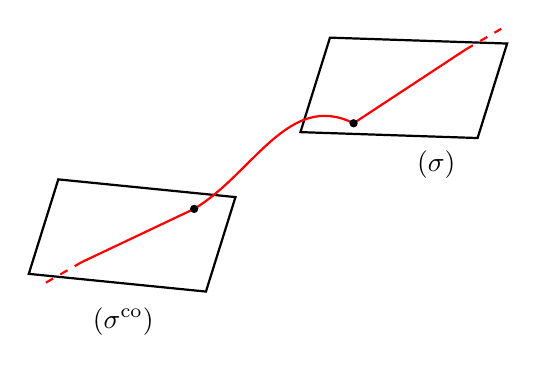
\begin{tikzpicture}[scale=0.75]
\draw[thick] (-4.2,-2.1)--(-1.2,-2.4)--(-0.7,-0.8)--(-3.7,-0.5)--cycle;
\draw[thick] (0.4,0.3)--(3.4,0.2)--(3.9,1.8)--(0.9,1.9)--cycle;
\draw[red,thick] (-3.3,-1.9)--(-1.4,-1.0);
\draw[dashed,red,thick] (-3.3,-1.9)--(-4.0,-2.3);
\draw[red,thick] (1.3,0.45)--(3.2,1.7);
\draw[dashed,red,thick] (3.2,1.7)--(3.8,2.05);
\draw[red,thick] (-1.4,-1.0) .. controls (-0.4,-0.4) and (0.2,1.0) .. (1.3,0.45);
\fill (-1.4,-1.0) circle (2pt);
\fill (1.3,0.45) circle (2pt);
\node at (-2.6,-2.9) {$\XX(\sigma^{\mathrm{co}})$};
\node at (2.7,-0.25) {$\XX(\sigma)$};
\end{tikzpicture}\\[3pt]
{\small $\XX(\sigma)\cong\XX(\sigma^{\mathrm{co}})$，沿其分裂轨迹（split loci）粘连，即 $t\leftrightarrow t^{-1}$。}
\end{center}

令 $X$ 记 $k$ 上一条带寻常二重点的 $\mathbb P^1$ 链，长度为 $(p-1)/2$。我们在 $X$ 的每个不可约分支上选取坐标 $T$，使得每个奇点在一个相交分支上对应 $0$、在另一分支上对应 $\infty$。我们称点 $0$ 与 $\infty$ 为\emph{标记点}（marked points）。

用伴权对 $\sigma,\sigma^{\mathrm{co}}$ 标号 $X$ 的各分支，并把相应的 $\mathbb P^1$ 记作 $X(\sigma|\sigma^{\mathrm{co}})$。各分支的次序由下述要求给出：若 $0<b<p-1$，则分支 $X(\sigma_{a,b}|\sigma_{a+b+1,p-3-b})$ 与分支 $X(\sigma_{a+b,p-1-b}|\sigma_{a+1,b-2})$ 相交。容易验证这样的标号恰有两种（而选取一种标号等同于选取链的一个端点）。

\begin{center}
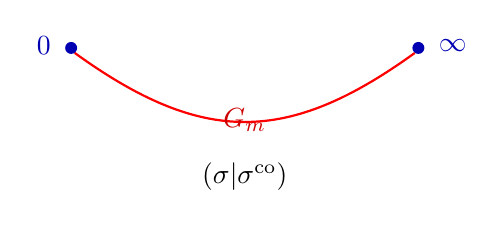
\begin{tikzpicture}[scale=0.9]
\draw[red,thick] (-2.4,0.4) .. controls (-0.6,-0.9) and (0.6,-0.9) .. (2.4,0.4);
\fill[blue!70!black] (-2.45,0.47) circle (2.4pt);
\fill[blue!70!black] (2.45,0.47) circle (2.4pt);
\node[blue!70!black,anchor=east] at (-2.6,0.5) {$0$};
\node[blue!70!black,anchor=west] at (2.6,0.5) {$\infty$};
\node[red!80!black] at (0,-0.55) {$\mathbb G_m$};
\node at (0,-1.35) {$\XX(\sigma|\sigma^{\mathrm{co}})$};
\end{tikzpicture}
\end{center}

这一构造的要点在于：利用我们对叠 $\XX(\sigma)$ 的显式描述，可以定义态射 $\pi:\XX_{\mathrm{red}}\to X$。我们仍满足于在非常 generic 的伴权对 $\sigma,\sigma^{\mathrm{co}}$ 情形给出描述。如下定义态射 $\pi_\sigma:\XX(\sigma|\sigma^{\mathrm{co}})\to X(\sigma|\sigma^{\mathrm{co}})$。按命题 7.2.11 把 $\XX(\sigma)$ 与 $[(\mathbb A^2\setminus\{0\})/\mathbb G_m]$ 等同，并取该处的坐标 $(t,x)$，把 $(t,x)$ 送到 $t$。再把 $\XX(\sigma^{\mathrm{co}})$ 与 $[(\mathbb A^2\setminus\{0\})/\mathbb G_m]$ 等同，并把 $(t,x)$ 送到 $t^{-1}$。注意按定义有 $\pi_{\sigma^{\mathrm{co}}}(x,t)=\pi_\sigma(x,t)^{-1}$。

对每个 Serre 权的伴权对 $\sigma,\sigma^{\mathrm{co}}$，我们在 $\pi_\sigma:\XX(\sigma|\sigma^{\mathrm{co}})\to X(\sigma|\sigma^{\mathrm{co}})$ 与 $\pi_{\sigma^{\mathrm{co}}}:\XX(\sigma|\sigma^{\mathrm{co}})\to X(\sigma|\sigma^{\mathrm{co}})$ 之中选取一个，使得这两个映射在 $X$ 的相邻分支的交点处一致。（这样的映射选取恰有两种，分别对应 $X$ 各分支的两种标号；两种可能的标号之间相差 $\det^{(p-1)/2}$ 的扭。）

\ysrc{282}
\begin{rem}{7.2.17}\label{rem:a4-7-2-17}
若 $\{\sigma,\sigma^{\mathrm{co}}\}$ 是非常 generic 的，则
\[
\XX(\sigma|\sigma^{\mathrm{co}})
\cong\bigl(\mathbb P^1_t\times[(\Spec k[x,y]/(xy))/(\mathbb G_m)_u]\bigr)
\setminus\bigl(0\times[\{x=0\}/\mathbb G_m]\cup\infty\times[\{y=0\}/\mathbb G_m]\bigr),
\]
其中 $\mathbb G_m$ 经 $u\cdot(x,y)=(u^2x,u^{-2}y)$ 作用。闭子叠 $\XX(\sigma)$ 由方程 $y=0$ 切出（此时 $x,t,u$ 对应命题 7.2.11 给出的 $\XX(\sigma)$ 描述中的同名变量），而 $\XX(\sigma^{\mathrm{co}})$ 由 $x=0$ 切出（此时 $y,t^{-1},u^{-1}$ 对应命题 7.2.11 给出的 $\XX(\sigma^{\mathrm{co}})$ 描述中出现的变量 $x,t,u$）。就这一显式描述而言，映射 $\XX(\sigma|\sigma^{\mathrm{co}})\to X(\sigma|\sigma^{\mathrm{co}})$ 就是到 $\mathbb P^1$ 因子的投影。
\end{rem}

\begin{rem}{7.2.18}\label{rem:a4-7-2-18}
可以验证：若 $\sigma_{a,b}$ 是满足 $b\ne0,p-1$ 的 Serre 权，则有同构
\[
\begin{aligned}
\XX(\sigma_{a,b})\cup\XX(\sigma_{a+b,p-1-b})
&\cong\bigl(\Spec k[t_1,t_2]/(t_1t_2)\times[\mathbb P^1_x/(\mathbb G_m)_u]\bigr)\\
&\qquad\setminus\bigl(\{t_1=0\}\times[0/\mathbb G_m]\cup\{t_2=0\}\times[\infty/\mathbb G_m]\bigr),
\end{aligned}
\]
其中 $\mathbb G_m$ 经 $u\cdot x=u^2x$ 作用在 $\mathbb P^1$ 上。

这里我们通过命题 7.2.11 把轨迹 $t_2=0$（相应地 $t_1=0$）与 $\XX(\sigma_{a,b})$（相应地 $\XX(\sigma_{a+b,p-1-b})$）等同，其中 $t_1$ 对应 $t$、$x$ 对应 $x$（相应地 $t_2$ 对应 $t$、$x$ 对应 $x^{-1}$）。
\end{rem}

\begin{center}
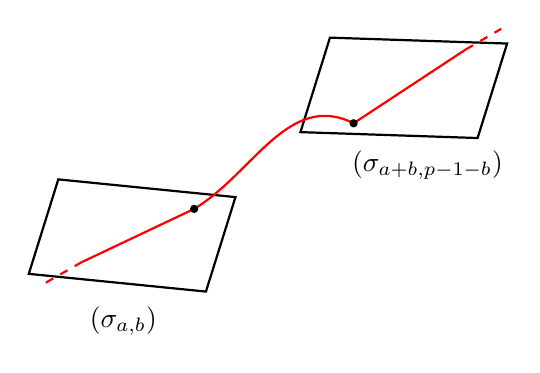
\begin{tikzpicture}[scale=0.75]
\draw[thick] (-4.2,-2.1)--(-1.2,-2.4)--(-0.7,-0.8)--(-3.7,-0.5)--cycle;
\draw[thick] (0.4,0.3)--(3.4,0.2)--(3.9,1.8)--(0.9,1.9)--cycle;
\draw[red,thick] (-3.3,-1.9)--(-1.4,-1.0);
\draw[dashed,red,thick] (-3.3,-1.9)--(-4.0,-2.3);
\draw[red,thick] (1.3,0.45)--(3.2,1.7);
\draw[dashed,red,thick] (3.2,1.7)--(3.8,2.05);
\draw[red,thick] (-1.4,-1.0) .. controls (-0.4,-0.4) and (0.2,1.0) .. (1.3,0.45);
\fill (-1.4,-1.0) circle (2pt);
\fill (1.3,0.45) circle (2pt);
\node at (-2.6,-2.9) {$\XX(\sigma_{a,b})$};
\node at (2.55,-0.25) {$\XX(\sigma_{a+b,p-1-b})$};
\end{tikzpicture}\\[3pt]
{\small $\XX(\sigma_{a,b})\cong\XX(\sigma_{a+b,p-1-b})$，沿其不可约轨迹（irreducible loci）粘连，即 $x\leftrightarrow x^{-1}$。}
\end{center}

由此容易看出，上述对态射 $\pi_\sigma$ 与 $\pi_{\sigma^{\mathrm{co}}}$ 的处方粘成态射 $\XX_{\mathrm{red}}\to X$。

\begin{rem}{7.2.19}\label{rem:a4-7-2-19}
$X$ 与态射 $\pi:\XX_{\mathrm{red}}\to X$ 的定义的动机如下。无论由一般原理，还是由我们对叠 $\XX(\sigma)$ 的显式描述，都容易看出 $X$ 的闭 $\bar\F_p$-点是半单的 $\bar\rho:\Gal_{\Q_p}\to\mathrm{GL}_2(\bar\F_p)$（行列式为 $\bar\varepsilon^{-1}$）。由 $\pi$ 的定义即知它在闭 $\bar\F_p$-点上诱导双射；我们把 $X$ 想成\ysrc{283}$\XX_{\mathrm{red}}$ 的「粗」模空间\footnote{我们给「粗」加上引号，因为态射 $\XX_{\mathrm{red}}\to X$ 并非例如 [Alp14] 技术意义下的粗模空间态射，甚至也不是一个 adequate 模空间态射（例如，因为它在底层拓扑空间上不是闭映射）。不过，它确实满足 [Alp14, Prop. 7.1.1] 的诸条件，特别地，它对从 $\XX_{\mathrm{red}}$ 到局部可分离代数空间的态射是初始的。}。在 $\bar\F_p$-点上，可以把态射 $\pi$ 看作把表示送到其半单化；更显式地说，分支 $X(\sigma|\sigma^{\mathrm{co}})$ 的标记点对应不可约的 $\bar\rho$，而删去标记点后所得的 $\mathbb G_m$ 参数化的是乘积固定、Frobenius 特征值由该 $\mathbb G_m$ 决定的特征之和。
\end{rem}

\begin{rem}{7.2.20}\label{rem:a4-7-2-20}
对 $F$ 的任意选取，都容易构造相应的模空间态射
\begin{equation}\tag{7.2.21}\label{eq:a4-7-2-21}
(\XX_{F,1})_{\mathrm{red}}\lra Y
\end{equation}
使其满足 [Alp14, Prop. 7.1.1] 的诸条件\tn{底本此处排印作「satisfying satisfying the conditions of [Alp14, Prop. 7.1.1] Indeed」，重复了一个 satisfying，且「]」后缺句点；依据为底本原样排印如此，疑为笔误，译文按原意处理。}。事实上，由于 $(\XX_{F,1})_{\mathrm{red}}$ 是形如 $[\Spec A/\mathbb G_m]$ 的全局商叠（其中 $\mathbb G_m$ 平凡地作用），取 $Y=\Spec A$，所得态射 (7.2.21) 甚至是 [Alp13] 意义下的好模空间态射。

进一步，由于 $\XX_{F,1}$ 可以写成 $[\Spf\hat A/\hat{\mathbb G}_m]$ 的形式，其中 $\Spf\hat A$ 是使 $\Spec A$ 加厚（thickens）的 adic 仿射形式概形、带有平凡的 $\hat{\mathbb G}_m$-作用；若再令 $\hat Y:=\Spf\hat A^{\hat{\mathbb G}_m}$，我们便得到态射 $\XX_{F,1}\to\hat Y$，它满足 [Alp14, Prop. 7.1.1] 诸条件的形式代数类比，并把 $\hat Y$ 实现为与 $\XX_{F,1}$ 自身相伴的形式模空间。

回到 $\mathrm{GL}_2(\Q_p)$ 情形。如已提及，我们预期上面构造的态射 $\XX_{\mathrm{red}}\to X$ 也容许一个形式加厚 $\XX\to\hat X$，且满足 [Alp14, Prop. 7.1.1] 诸条件的形式代数类比。另一方面，若 $F\ne\Q_p$ 且 $d\ge2$，甚至当 $F=\Q_p$ 而 $d>2$ 时，我们不预期存在有趣的模空间态射 $\XX_{F,d}\to\hat Y$ 或 $(\XX_{F,d})_{\mathrm{red}}\to Y$。更精确地说，在这些情形我们预期：从 $\XX_{F,d}$ 到局部可分离形式代数空间的任何态射都经过行列式映射 $\XX_{F,d}\to\XX_{F,1}$。
\end{rem}

\subsubsection*{7.2.22.\quad 一些开子叠}

固定非常 generic 的 Serre 权伴权对 $\sigma,\sigma^{\mathrm{co}}$，并用 $U(\sigma|\sigma^{\mathrm{co}})$ 记 $|X(\sigma|\sigma^{\mathrm{co}})|$ 中删去标记点 $0,\infty$ 所得到的开子集。则 $U(\sigma|\sigma^{\mathrm{co}})$ 也是 $|X|$ 中的开集；我们以 $\mathcal U(\sigma|\sigma^{\mathrm{co}})$（有时简记 $\mathcal U$）记 $U(\sigma|\sigma^{\mathrm{co}})$ 的原像，把它看作 $\XX$ 的开子叠。于是 $\mathcal U_{\mathrm{red}}=\mathcal U(\sigma|\sigma^{\mathrm{co}})_{\mathrm{red}}$ 是 $\XX(\sigma|\sigma^{\mathrm{co}})$ 中删去对应不可约 $\bar\rho$ 的轨迹（由两个闭点组成）所得到的（稠密）开子叠；更精确地说，$\mathcal U_{\mathrm{red}}$ 是其两个闭子叠 $\mathcal U\cap\XX(\sigma)$ 与 $\mathcal U\cap\XX(\sigma^{\mathrm{co}})$ 之并。

就注 7.2.17 给出的 $\XX(\sigma|\sigma^{\mathrm{co}})$ 的描述而言，$U(\sigma|\sigma^{\mathrm{co}})_{\mathrm{red}}$ 由
\[
\bigl[(\mathbb G_m\times\Spec k[x,y]/(xy))/\mathbb G_m\bigr]
=[\Spec k[t^{\pm1},x,y]/(xy)/\mathbb G_m]
\]
给出，$\mathbb G_m$-作用为
\[
u\cdot(x,y)=(u^2x,u^{-2}y).
\]

\ysrc{284}
\begin{center}
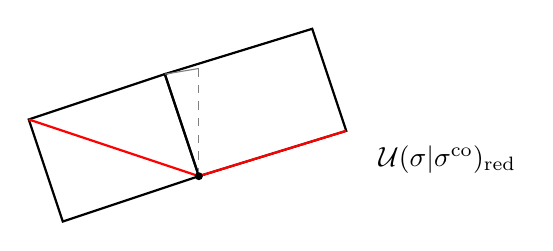
\begin{tikzpicture}[scale=0.72]
\draw[thick] (-3.0,-0.2)--(-0.6,0.6)--(0.0,-1.2)--(-2.4,-2.0)--cycle;
\draw[thick] (-0.6,0.6)--(2.0,1.4)--(2.6,-0.4)--(0.0,-1.2)--cycle;
\draw[red,thick] (-3.0,-0.2)--(0.0,-1.2)--(2.6,-0.4);
\draw[gray,dashed] (0.0,-1.2)--(0.0,0.7);
\draw[gray] (0.0,0.7)--(-0.6,0.6);
\fill (0.0,-1.2) circle (2pt);
\node[anchor=west] at (3.0,-0.9) {$\mathcal U(\sigma|\sigma^{\mathrm{co}})_{\mathrm{red}}$};
\end{tikzpicture}
\end{center}

以形变理论（deformation theory）论证建立在此描述之上，我们可以把 $\mathcal U$ 显式地描述为
\begin{equation}\tag{7.2.23}\label{eq:a4-7-2-23}
\mathcal U(\sigma|\sigma^{\mathrm{co}})
=\bigl[\Spf\mathcal O[s,t^{\pm1},x,y]^{\wedge}/\hat{\mathbb G}_m\bigr],
\end{equation}
其中 hat 指 $(p,s,xy)$-adic 完备化，而 $\hat{\mathbb G}_m$-作用由
\[
u\cdot(s,t,x,y)=(s,t,u^2x,u^{-2}y)
\]
给出。这里 $\mathcal U\cap\XX(\sigma)$ 是轨迹 $\varpi=s=y=0$，$\mathcal U\cap\XX(\sigma^{\mathrm{co}})$ 由 $\varpi=s=x=0$ 给出（与命题 7.2.11 中描述的等同由 $y\mapsto x^{-1}$、$t\mapsto t^{-1}$ 给出）。

\begin{center}
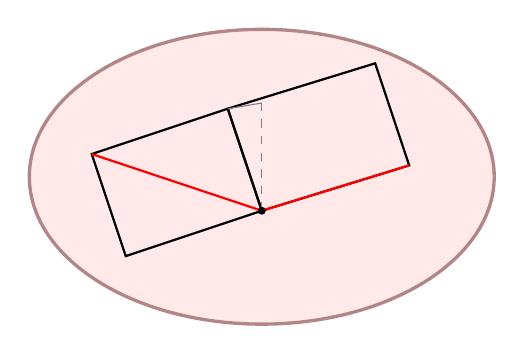
\begin{tikzpicture}[scale=0.72]
\fill[pink!35] (0,-0.6) ellipse (4.1 and 2.6);
\draw[pink!70!black,very thick] (0,-0.6) ellipse (4.1 and 2.6);
\draw[thick] (-3.0,-0.2)--(-0.6,0.6)--(0.0,-1.2)--(-2.4,-2.0)--cycle;
\draw[thick] (-0.6,0.6)--(2.0,1.4)--(2.6,-0.4)--(0.0,-1.2)--cycle;
\draw[red,thick] (-3.0,-0.2)--(0.0,-1.2)--(2.6,-0.4);
\draw[gray,dashed] (0.0,-1.2)--(0.0,0.7);
\draw[gray] (0.0,0.7)--(-0.6,0.6);
\fill (0.0,-1.2) circle (2pt);
\end{tikzpicture}\\[3pt]
{\small $\mathcal U(\sigma|\sigma^{\mathrm{co}})_{\mathrm{red}}$ 位于形式光滑叠 $\mathcal U(\sigma|\sigma^{\mathrm{co}})$ 内部（粉色区域示意后者）。}
\end{center}

\subsubsection*{7.2.24.\quad 更多开子叠}

如注 7.2.18 那样，取满足 $b\ne0,p-1$ 的 Serre 权 $\sigma_{a,b}$。并集 $\XX(\sigma_{a,b})\cup\XX(\sigma_{a+b,p-1-b})$ 含唯一的闭点，其相应的伽罗瓦表示 $\bar\rho$ 不可约。若从该并中删去分裂轨迹（就注 7.2.18 的显式描述而言，即删去轨迹 $x=0$ 与 $x=\infty$），我们得到 $\XX_{\mathrm{red}}$ 的一个含 $\bar\rho$ 的开子集 $\mathcal V_{\mathrm{red}}$，它有显式描述
\[
\mathcal V_{\mathrm{red}}=[\Spec k[t_1,t_2]/(t_1t_2)/\mu_2],
\]
其中 $\mu_2$-作用是平凡的。

\ysrc{285}
若以 $\mathcal V$ 记 $\XX$ 中对应 $\XX_{\mathrm{red}}$ 的开子集 $\mathcal V_{\mathrm{red}}$ 的开子叠，则形变理论论证表明 $\mathcal V$ 有如下描述：
\[
\mathcal V\cong\bigl[\Spf\mathcal O[a,t_1,t_2]^{\wedge}/\mu_2\bigr],
\]
其中 hat 指 $(p,a,t_1t_2)$-adic 完备化，而 $\mu_2$-作用再次是平凡的。

\subsection{$\mathrm{GL}_2(\Q_p)$ 的 Banach 情形 —— II. 证明梗概}

本节我们勾勒期望 7.2.1 的证明。

\subsubsection*{7.3.1.\quad $L_\infty$ 的构造}

我们先定义 $\mathrm{GL}_2(\Q_p)$-表示的 pro-凝聚层 $L_\infty$。本质上，它是 Colmez 的 $\mathrm{GL}_2(\Q_p)$-表示 $D^\natural\boxtimes\mathbb P^1$ 的自然推广。[Col10b] 的一部分论证在我们的设定下几乎原样通过，但另一些则需要更认真的改造。（出现的一些主要困难是：Colmez 的 $D^\natural$ 与 $D^{\mathrm{nr}}$ 与平坦基变换不相容，故凡涉及它们的论证都须重做；此外，当处理一般系数的 $(\varphi,\Gamma)$-模时，格的商不必是字面意义下有限的模，故凡涉及这类有限性陈述的论证也须重做。）

首先注意，按定义 $\XX$ 上存在万有的秩 2 $(\varphi,\Gamma)$-模 $D$。我们发觉在其定义中引入一个扭较为方便，方式如下。若 $A$ 是有限型的 $\mathcal O/\varpi^a$-代数，则态射 $\Spec A\to\XX$ 对应一个带 $A$-系数、行列式为逆分圆特征的秩 2 $(\varphi,\Gamma)$-模，且该 $(\varphi,\Gamma)$-模的构造与 $A$ 中的基变换相容。我们以 $D_A$ 记该 $(\varphi,\Gamma)$-模按分圆特征所作的扭，于是 $D_A$ 的行列式等于分圆特征（而非其逆）。

我们处理全分圆扩张 $\Q_p(\zeta_{p^\infty})/\Q_p$ 的 $(\varphi,\Gamma)$-模，于是 $D_A$ 是环
\[
\mathbf A_A=A((T))
\]
上的秩 2 投射模，配有交换的（$A$-线性的半线性）$\varphi$ 与 $\Gamma$ 作用，其中
\[
\varphi(1+T)=(1+T)^p,
\]
\[
\gamma(1+T)=(1+T)^{\varepsilon(\gamma)}
\]
对任意 $\gamma\in\Gamma$ 成立（其中 $\varepsilon$ 照例是 $p$-进分圆特征）。此外还有 $\varphi$ 的一个左逆 $\psi:D_A\to D_A$；它是 $A$-线性满射、与 $\Gamma$ 交换，并满足
\[
\psi(\varphi(a)m)=a\psi(m),\qquad
\psi(a\varphi(m))=\psi(a)m
\]
对任意 $a\in\mathbf A_A$、$m\in D_A$ 成立。

\ysrc{286}
仿照 Colmez，我们利用 $\varphi,\psi,\Gamma$ 在 $D_A$ 上的作用显式地构造一个 $\mathrm{GL}_2(\Q_p)$-表示。记 $P^+$ 为半群 $\bigl(\begin{smallmatrix}\Z_p\setminus\{0\}&\Z_p\\0&1\end{smallmatrix}\bigr)$，$P$ 为群 $\bigl(\begin{smallmatrix}\Q_p^\times&\Q_p\\0&1\end{smallmatrix}\bigr)$。则 $P^+$ 通过连续映射
\[
\begin{pmatrix}p^ka&b\\0&1\end{pmatrix}z=(1+T)^b\varphi^k\circ\sigma_a(z)
\]
作用在 $D_A$ 上，其中 $a\in\Z_p^\times$、$b\in\Z_p$、$k\in\Z_{\ge0}$，而 $\sigma_a\in\Gamma$ 记满足 $\varepsilon(\sigma_a)=a$ 的元素。

$P^+$ 自然地作用在 $\Z_p$ 上（相应地 $P$ 自然地作用在 $\Q_p$ 上），作用为 $\begin{pmatrix}a&b\\0&1\end{pmatrix}x=ax+b$；如 [Col10c, §3.1] 所述，这一作用可用来在 $\Z_p$ 上定义 $A$-模的 $P^+$-等变层 $\mathcal U\mapsto D_A\boxtimes\mathcal U$。具体做法是：令 $D_A\boxtimes\mathbf Z_p$ 为 $D_A$ 自身；对任意 $i\in\Z_p$ 与 $k\ge0$，$D_A\boxtimes(i+p^k\Z_p)$ 在 $i+p^k\Z_p$ 上的截面定义为 $\begin{pmatrix}p^k&i\\0&1\end{pmatrix}D_A\subseteq D_A$。限制映射 $\operatorname{Res}_{i+p^k\Z_p}:D_A\boxtimes\mathbf Z_p\to D_A\boxtimes(i+p^k\Z_p)$ 由
\[
\begin{pmatrix}1&i\\0&1\end{pmatrix}\circ\varphi^k\circ\psi^k\circ\begin{pmatrix}1&-i\\0&1\end{pmatrix}
\]
给出。于是特别有 $D_A\boxtimes\mathbf Z_p^\times=D_A^{\psi=0}$。

给定 $\Z_p$ 的紧开子集之间的仿射线性映射 $f:U\to V$，有诱导映射 $f_*:M\boxtimes U\to M\boxtimes V$。此定义立刻推广到局部仿射线性的连续映射，再通过取极限推广到可被仿射线性映射适当逼近的函数。特别地，它适用于 $\Z_p^\times$ 上的映射 $z\mapsto1/z$；于是可用该映射把 $D_A\boxtimes\mathbf Z_p$ 沿 $D_A\boxtimes\mathbf Z_p^\times$ 与自身粘成 $\mathbb P^1(\Z_p)(=\mathbb P^1(\Q_p)=\Q_p\cup\{\infty\})$ 上的层。我们以 $D_A\boxtimes\mathbb P^1$ 记该层的整体截面；由函子性，它们带有 $\mathrm{GL}_2(\Q_p)$ 的作用（中心特征平凡）。

由于 $\Q_p$ 是 $\mathbb P^1(\Z_p)$ 的开子集，我们也可以取 $D_A\boxtimes\mathbb P^1$ 在 $\Q_p$ 上的截面，得到一个 $B$-表示，记作 $D_A\boxtimes\Q_p$。展开定义可知，$D_A\boxtimes\Q_p$ 有作为逆极限 $\varprojlim_\psi D_A$ 的显式描述。

$\mathrm{GL}_2(\Q_p)$ 在 $D_A\boxtimes\mathbb P^1$ 上的作用与 $A$ 中的平坦基变换相容，但 $D_A\boxtimes\mathbb P^1$ 并非我们所寻求的 $L_\infty$。这在 [Col10b] 的原设定中已很明显：在那里 $D_A\boxtimes\mathbb P^1$ 实现的不是局部 Langlands 对应，而是该对应由其对偶（带扭）所作的扩张。（关于这一现象在我们设定下的预期推广，见下文 7.3.22 小节。）因此我们（仍仿照 Colmez）把 $L_\infty$ 构造为 $D_A\boxtimes\mathbb P^1$ 的子表示。

为此令 $\mathbf A_A^+=A[[T]]$，它从 $\mathbf A_A$ 继承 $\varphi,\psi,\Gamma$ 的作用。可以证明 $D_A$ 含有极小的 $\psi$-稳定 $\mathbf A_A^+$-格 $D_A^\natural$（「格」意即：它作为 $\mathbf A_A^+$-模有限生成，且在 $\mathbf A_A$ 上张成 $D_A$），其构造与平坦基变换相容。有自然的限制映射
\[
\operatorname{Res}_{\Q_p}:D_A\boxtimes\mathbb P^1\lra D_A\boxtimes\Q_p,
\]
并令
\[
D_A^\natural\boxtimes\mathbb P^1
:=\bigl\{z\in D_A\boxtimes\mathbb P^1,\ \operatorname{Res}_{\Q_p}(z)\in D_A^\natural\boxtimes\Q_p\bigr\},
\]
其中 $D_A^\natural\boxtimes\Q_p:=\varprojlim_\psi D_A^\natural$。

结果是：$D_A^\natural\boxtimes\mathbb P^1$ 是 $D_A\boxtimes\mathbb P^1$ 中的 $\mathrm{GL}_2(\Q_p)$-稳定格，但这完全不显然；事实上，即使在 [Col10b] 的原设定中，$D_A^\natural\boxtimes\mathbb P^1$ 在 $D_A\boxtimes\mathbb P^1$ 中是开的这一点也完全不显然。（这里「格」取 [Dri06] 的意义：$A$ 上 Tate 模中的格是开 $A$-子模 $L$，满足：若 $U\subseteq L$ 是开的，则 $L/U$ 是有限生成 $A$-模。）

证明 $D_A^\natural\boxtimes\mathbb P^1$ 是 $\mathrm{GL}_2(\Q_p)$-稳定格相当复杂；它涉及（通过考虑完备局部环）把情形归结为 $A$ 是 Artinian 的情形，

% 本片止于印刷页 286 页末（§7.3.1），续片自 PDF 300 页起
